\chapter{TỔNG QUAN} % Tên của chương

\label{Chapter2} % Để trích dẫn chương này ở chỗ nào đó trong bài, hãy sử dụng lệnh \ref{Chapter1} 
\section{Dataset sử dụng}
Việc sử dụng nhiều dataset khác nhau cho phép đa dạng dữ liệu
đầu vào và kiểm tra được tính linh hoạt của mô hình trong nhiều trường hợp khác nhau.
\subsection{Emotional attitude captioning dataset}
Dataset sử dụng trong bài có 3840 ảnh khác nhau, được lấy từ IMDB dataset. Mỗi ảnh được gán nhãn với một số trạng thái như là "laughing", "flirting", "kissing", "angry", "happy", ...\cite{web:4}. 

\begin{figure}[h!]
	\centering
	
\includegraphics[width=10cm]{nm0000202_rm1918408960_1974-9-10_2008.jpg}
	\caption{Gán nhãn: Two guys are looking on each other.}
\end{figure} 
\subsection{Flickr8}
Dataset được lấy trên trang web Kaggle \cite{web:8}.

\section{Mô hình CNN}
CNN (Convolutional Neural Network) là một mô hình Deep learning để xử lí dữ liệu ở dạng lưới như là hình ảnh, được thiết kế để học một cách tự động và thích ứng với hệ thống phân cấp không gian của các tính năng, từ pattern thấp tới cao.\cite{yamashita2018convolutional}

Nó sử dụng một kĩ thuật đặc biệt gọi là tích chập (Convolution), một phép toán trên hai phương trình để đưa ra phương trình thứ ba mô tả cách hình dạng của một phương trình bị thay đổi bởi phương trình còn lại.\cite{web:2}

\begin{figure}[h!]
	\centering
	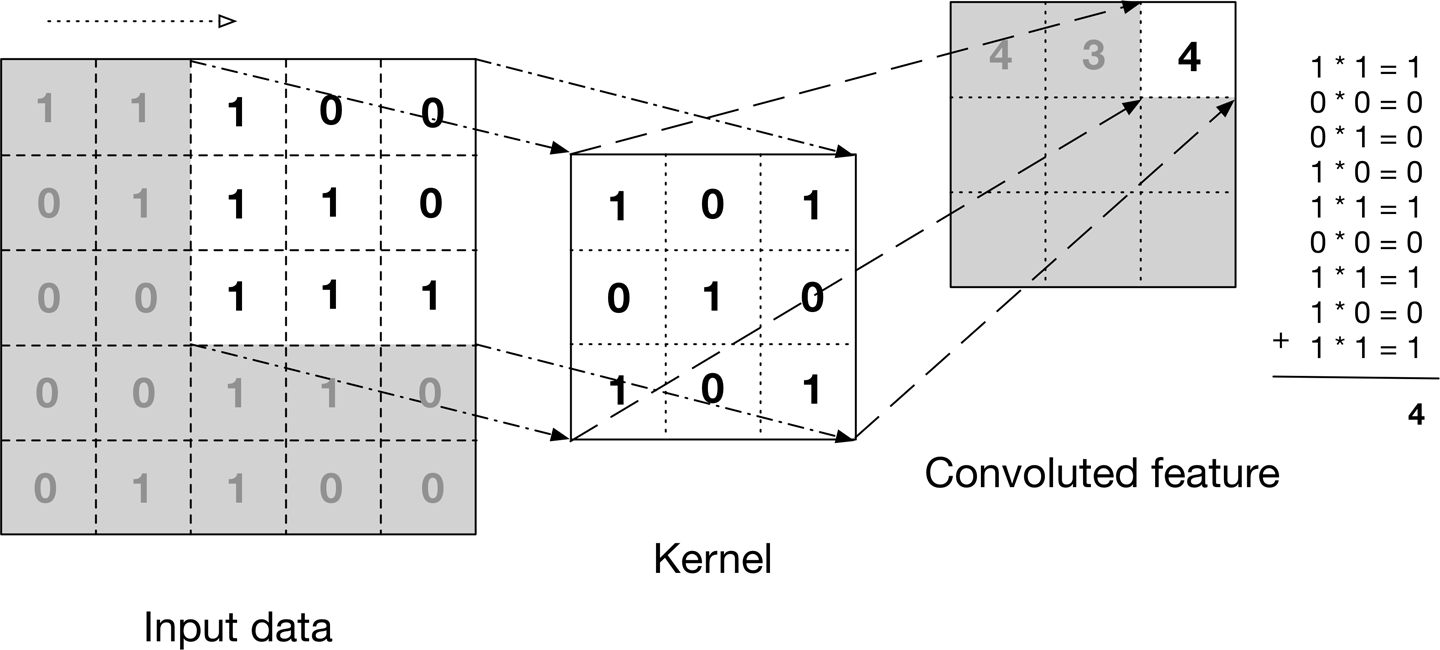
\includegraphics[width=14cm]{convolution1.png}
	\caption{Tích chập.}
\end{figure}  

Cấu trúc của CNN thường gồm ba loại lớp:
\begin{itemize}
	\item Convolution
	\item Pooling
	\item Fully connected 
\end{itemize} 

\begin{figure}[h!]
	\centering
	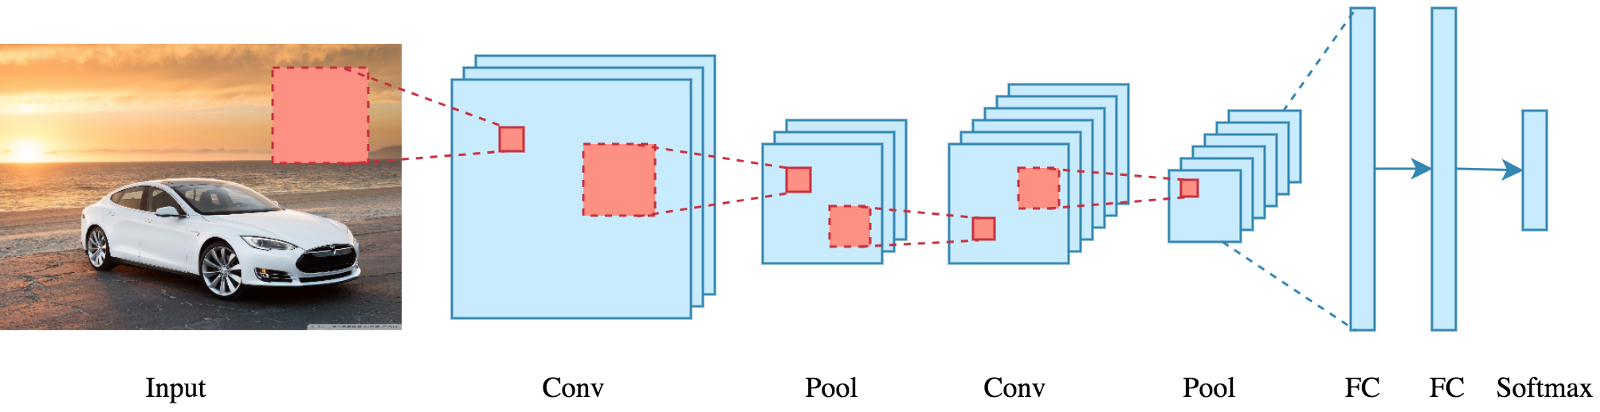
\includegraphics[width=15cm]{convo_layers.png}
	\caption{Các lớp của mô hình CNN.}
\end{figure} 

Khi đầu vào là một ảnh, mỗi lớp sẽ tạo ra các hàm kích hoạt sau đó tiếp tục được đưa vào lớp tiếp theo. Lớp đầu tiên thường sẽ trích xuất ra đặc điểm cơ bản của ảnh như các cạnh ngang và chéo. Đầu ra này sẽ được đưa vào lớp tiếp theo để xác định các góc và cạnh tổ hợp. Càng đưa vào nhiều lớp sâu hơn, ta càng tìm được các đặc điểm phức tạp như vật thể, mặt, ...\cite{web:2}.

\newpage
\subsection{Convolutional layer}
\subsubsection{a) Kernel}
Kernel là một ma trận vuông có kích thước KxK với K là các số lẻ. Ma trận X tích chập với kernal sẽ được ma trận Y.
\begin{figure}[h!]
	\centering
	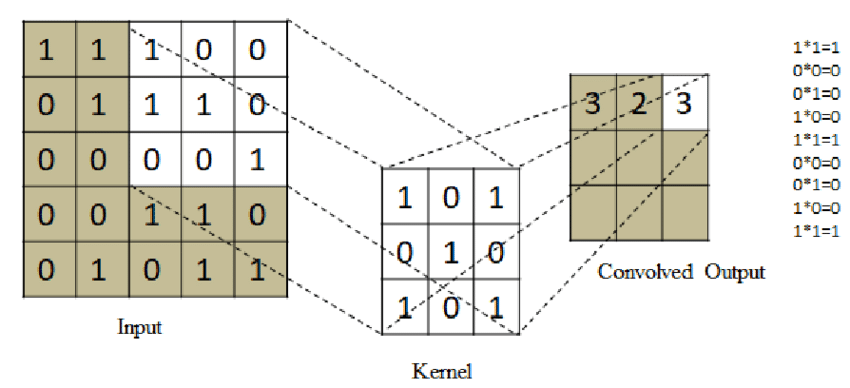
\includegraphics[width=13cm]{kernal_convo.png}
	\caption{Phép tính với kernel.}
\end{figure} 

\subsubsection{b) Padding}
Sau phép biến đổi Convolution, ma trận Y sẽ có kích thước nhỏ hơn X. Nếu muốn ma trận Y có cùng kích thước với X thì ta cần thêm giá trị 0 vào viền ngoài ma trận X trước khi thực hiện phép tính. Việc thêm viền ngoài này được gọi là Padding.

\begin{figure}[h!]
	\centering
	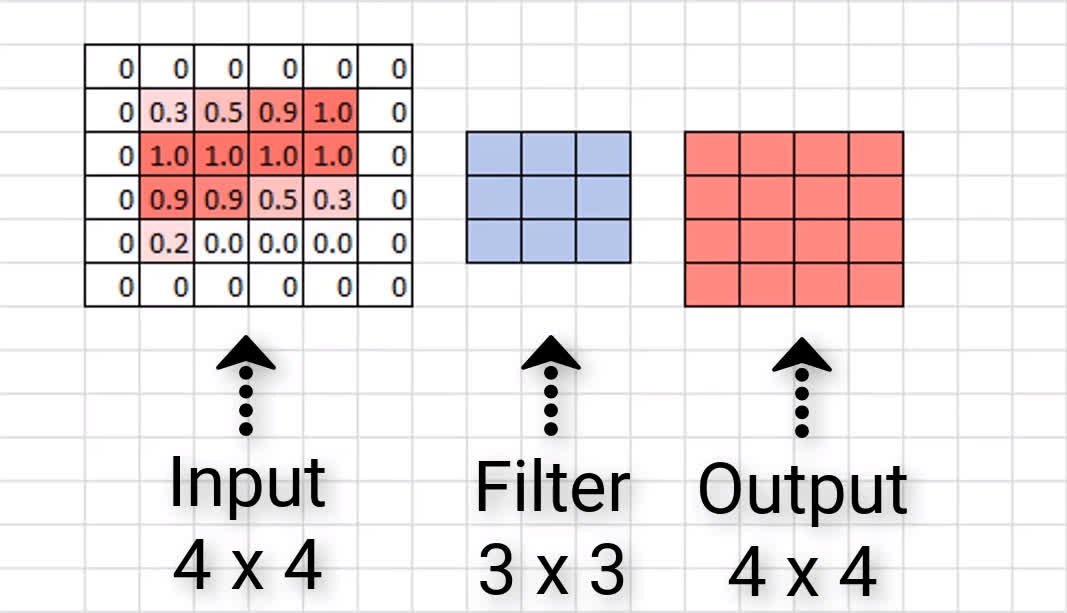
\includegraphics[width=11cm]{padding_convo.jpg}
	\caption{Thêm padding.}
\end{figure} 

\subsubsection{c) Stride}
Nếu thực hiện phép tích chập lần lượt trên các phần tử $x_{i,j}$, $x_{i,j+1}$, ... cho đến hết ma trận thì khi đó Stride là 1. Stride bằng n thì ta sẽ thực hiện phép tính trên các phần tử $x_{i,j}$, $x_{i,j+n}$, ...

\begin{figure}[h!]
	\centering
	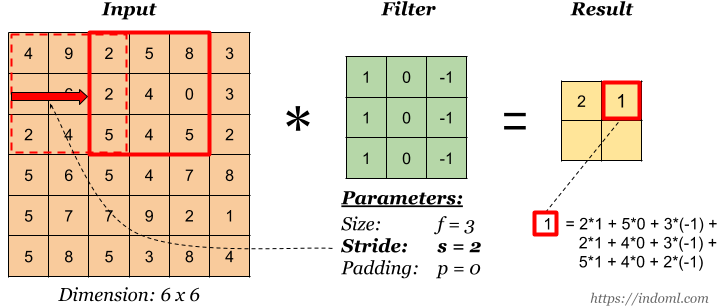
\includegraphics[width=13cm]{stride_convo.png}
	\caption{Stride = 2.}
\end{figure} 

\subsection{Polling layer}
Pooling layer thường được dùng giữa các convolutional layer, để giảm kích thước dữ liệu nhưng vẫn giữ được các thuộc tính quan trọng. Việc giảm kích thước dữ liệu giúp giảm các phép tính toán
trong model.

Bên cạnh đó, với phép pooling kích thước ảnh giảm, do đó lớp convolution học được các vùng có kích thước lớn hơn. Ví dụ như ảnh kích thước 224*224 qua pooling về 112*112 thì vùng 3*3 ở ảnh 112*112 tương ứng với vùng 6*6 ở ảnh ban đầu. Vì vậy qua các pooling thì kích thước ảnh nhỏ đi và convolutional layer sẽ học được các thuộc tính lớn hơn.

\begin{figure}[h!]
	\centering
	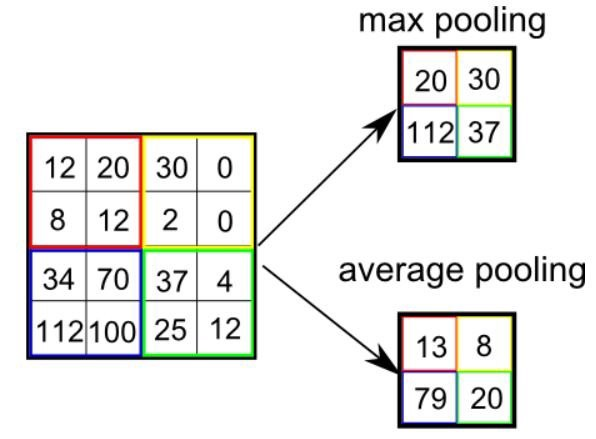
\includegraphics[width=9cm]{polling_convo.png}
	\caption{Hai loại polling.}
\end{figure} 

\newpage
\subsection{Fully connected layer}
Sau khi qua Convolution layers và Polling layers thì đầu ra vẫn là một ma trận nhiều hàng nhiều cột. Trước khi đưa dữ liệu vào lớp Fully connected ta cần phải biến đổi dữ liệu thành dạng nhiều hàng một cột.

\begin{figure}[h!]
	\centering
	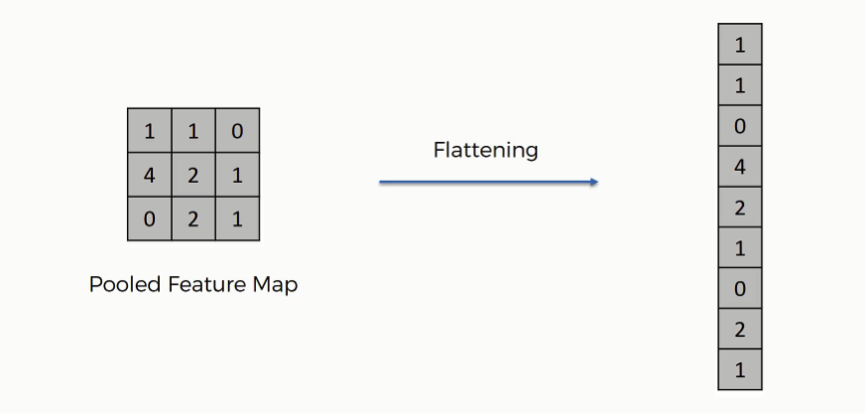
\includegraphics[width=13cm]{flatten.png}
	\caption{Flattening.}
\end{figure} 

Lớp Fully connected đề cập tới mạng nơ-ron trong đó mỗi nơ-ron áp dụng một phép biến đổi tuyến tính cho vecto đầu vào thông qua ma trận trọng số. Kết quả là tất cả đầu vào của vecto đầu vào đều có ảnh hưởng đến tất cả đầu ra của vecto đầu ra \cite{web:3}.

\begin{figure}[h!]
	\centering
	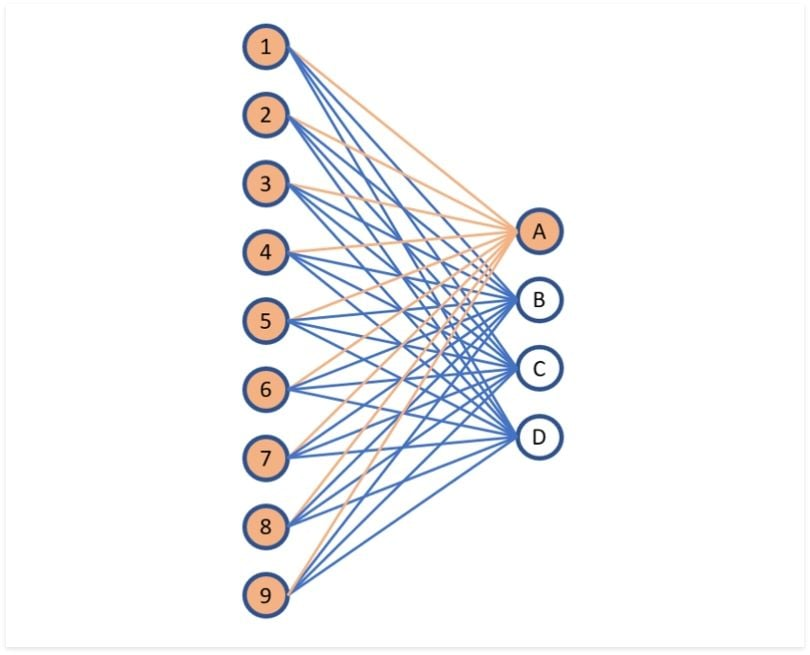
\includegraphics[width=11cm]{fully_convo.jpg}
	\caption{Fully connected layer.}
\end{figure} 

Trong quá trình đào tạo, để tránh mô hình bị overfitting (mô hình dự đoán có kết quả chính xác rất cao đối với tập dữ liệu cho trước nhưng khi áp dụng với tập dữ liệu bên ngoài thì độ chính xác giảm một cách đáng kể), một vài nơ-ron bị loại bỏ một cách ngẫu nhiên. Việc này giúp vecto đầu ra không bị phụ thuộc hoàn toàn vào giá trị của vecto đầu vào, kỹ thuật này được gọi là drop out.

\begin{figure}[h!]
	\centering
	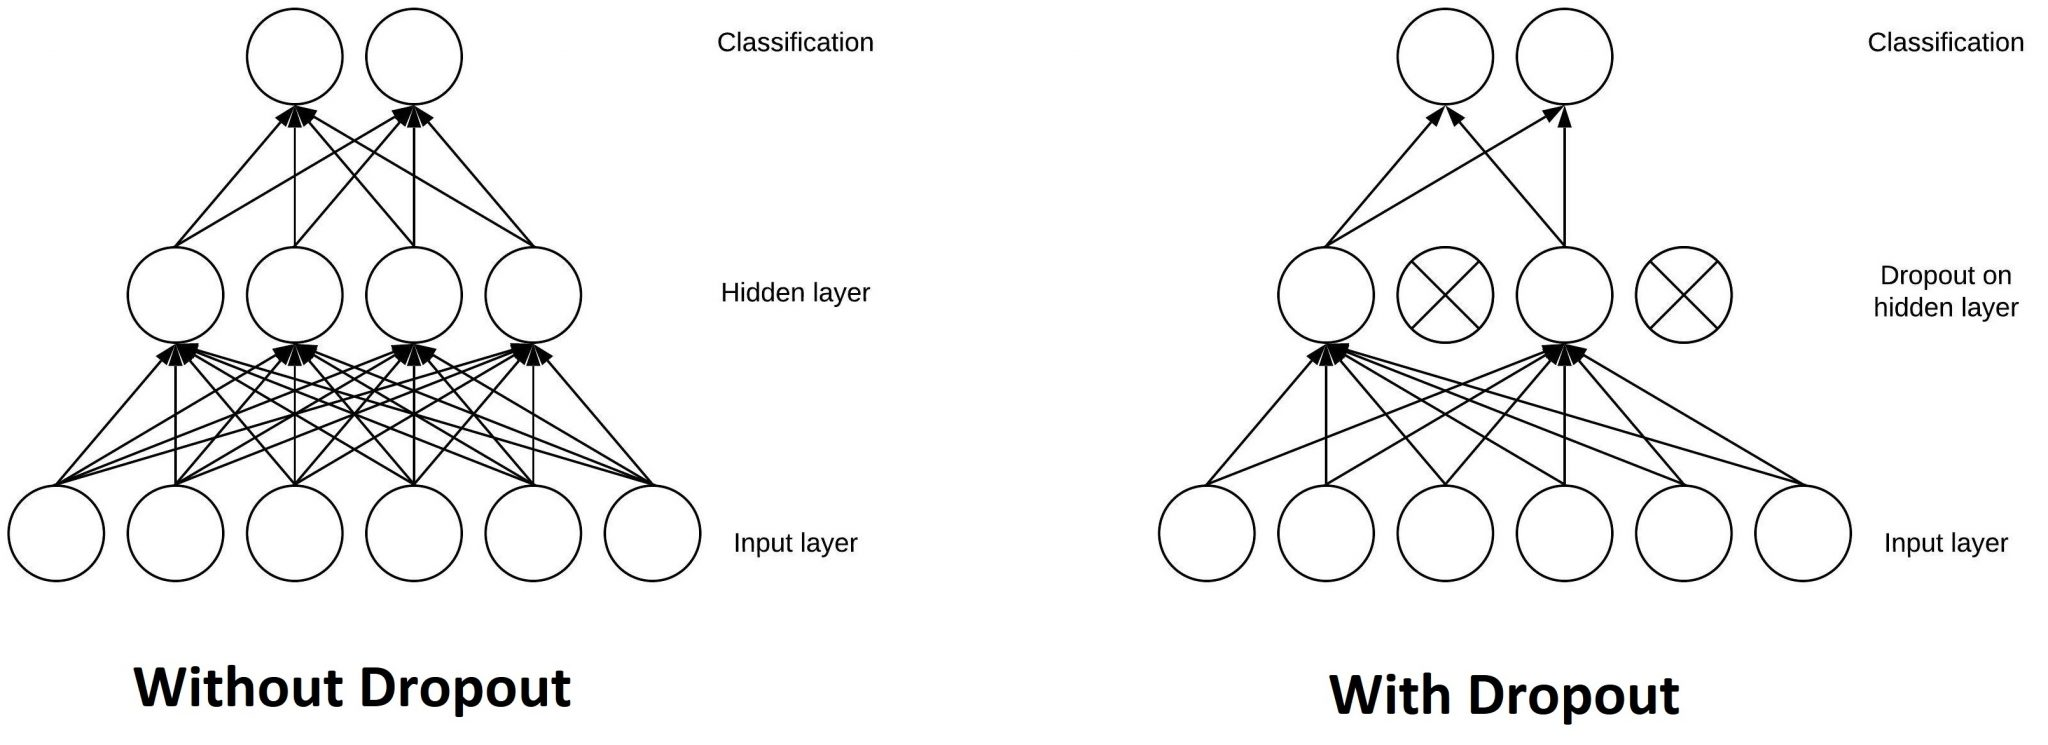
\includegraphics[width=12cm]{drop_out.jpg}
	\caption{Drop out.}
\end{figure} 

\newpage
\section{Mô hình RNN}
Như đã biết, Neural Network gồm 3 phần: Input layer, Hidden layer và Output layer. Các đầu vào và đầu ra trong mạng này đều độc lập với nhau do đó mô hình này không phù hợp với những bài toán dạng chuỗi như mô tả, hoàn thành câu,... vì những dự đoán tiếp theo sẽ phụ thuộc vào vị trí trước của nó. RNN ra đời với ý tưởng chính là để giải quyết các bài toán đó.

RNN (Recurrent Neural Network) là một kiến trúc mạng nơ-ron có khả năng xử lý và phân tích các dữ liệu tuần tự. Trong RNN, mỗi nút (hoặc đơn vị) thực hiện các phép tính trên đầu vào hiện tại và trạng thái ẩn được truyền tiếp từ đơn vị trước đó.

\begin{figure}[h!]
	\centering
	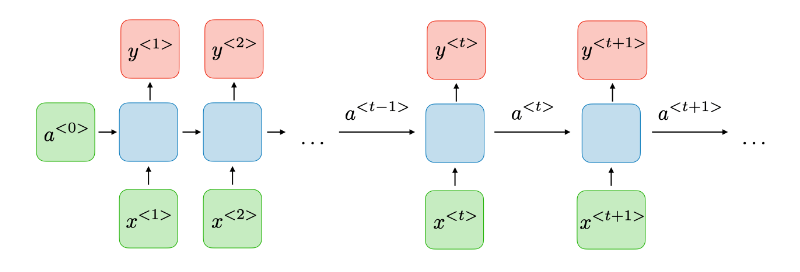
\includegraphics[width=14cm]{RNN1.png}
	\caption{Recurrent neural network.}
\end{figure} 

RNN được chia ra thành bốn loại:
\begin{itemize}
	\item One to one:
	Đây còn được gọi là mạng Neural thuần túy. Nó xử lý một kích thước cố định của đầu vào với kích thước cố định của đầu ra, nơi chúng độc lập với thông tin đầu ra trước đó. 
	\item One to many:
	Nó xử lý một kích thước cố định của thông tin làm đầu vào cung cấp một chuỗi dữ liệu làm đầu ra.
	\item Many to one:
	Bài toán có nhiều input nhưng chỉ có 1 output, ví dụ bài toán phân loại hành động trong video, input là nhiều ảnh (frame) tách ra từ video, ouptut là hành động trong video.
	\item Many to many:
	Bài toán có nhiều input và nhiều output, ví dụ bài toán dịch từ tiếng Anh sang tiếng Việt, input là 1 câu gồm nhiều chữ: “I love Vietnam” và output cũng là 1 câu gồm nhiều chữ “Tôi yêu Việt Nam”.
\end{itemize}

\begin{figure}[h!]
	\centering
	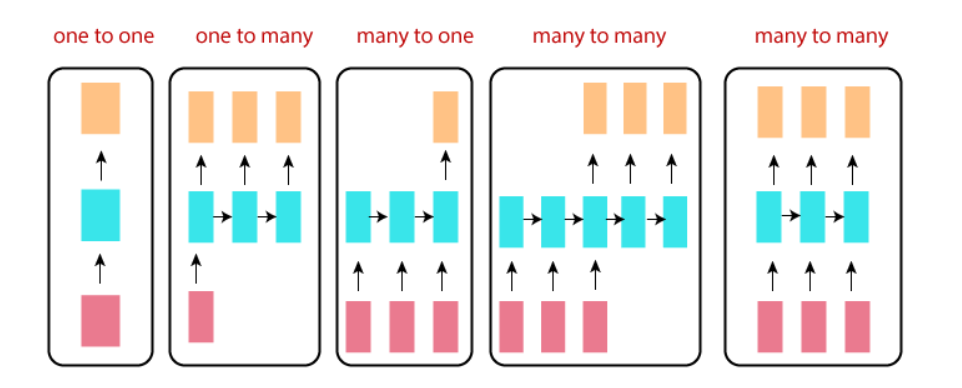
\includegraphics[width=13cm]{cacRNN.png}
	\caption{Các loại RNN.}
\end{figure} 

Tuy nhiên mô hình RNN cũng tồn tại những hạn chế rõ ràng \cite{web:5}:
\begin{itemize}
	\item RNN có nhiệm vụ đưa thông tin đi kịp thời. Tuy nhiên, việc truyền tất cả các thông tin này là một việc khá khó khăn bởi thời gian quá dài. Điều đó dẫn đến RNN có thể gặp phải vanishing gradient (hệ số phản hồi không thể thay đổi khi các trạng thái mới đi qua mô hình). Việc này đồng nghĩa với việc mô hình không thể học được từ thông tin do đó kết quả đưa ra sẽ bị sai.
	\item Không thể mô hình hóa các thông tin dài hạn.
	\item RNN yêu cầu đầu vào mỗi chuỗi có độ dài bằng nhau do đó khó khăn trong việc xử lý các chuỗi có độ dài khác nhau. 
\end{itemize}

\newpage
\section{Mô hình LSTM}
Xuất phát từ những nhược điểm kể trên của RNN truyền thống, mô hình LSTM (Long Short – Term Memory) đã được ra đời. Dù mô hình LSTM có những kết nối phản hồi như mô hình RNN, nhưng quá trình xử lý không chỉ các điểm dữ liệu đơn lẻ mà là toàn bộ chuỗi dữ liệu. Từ đó kết quả trở lên lý tưởng hơn để xử lý và dự đoán dữ liệu, LSTM có nhiều ứng dụng trong nhận dạng chữ viết tay, nhận diện giọng nói, phát hiện giọng nói, trò chơi,...\cite{hochreiter1997long}

\subsection{Short term và Long term memory}
Short term memory là quá trình học từ những trạng thái được lưu trữ thông tin của layer trước tới layer sau khi thông tin đó được mang qua state nhất định. Nó là giá trị lưu trữ để tính toán đầu ra dự đoán đối với giá trị input. Short term memory của mô hình RNN sẽ tiếp tục liện tục qua nhiều state và khó kiểm soát và gặp vấn đề.

Long term memory là quá trình xác định thông tin đi xa hơn sau hàng ngàn state và sẽ được sử dụng khi cần. Giá trị long term memory sẽ được lưu trữ mới mỗi khi mộtshort term memory tính toán ra state tiếp theo của layer.

Để không xảy ra hiện tượng vanishing gradient, hàm kích hoạt được sử dụng là tanh và sigmoid. Giá trị đầu ra của hàm tanh bị giới hạn từ -1 < y < 1; đầu ra của hàm sigmoid giới hạn từ 0 < y < 1 sẽ điều chỉnh đầu ra như một hàm xác suất để dự đoán giống như các bài toán của Machine Learning. Kể cả đầu vào là một hình ảnh với ma trận hệ số màu thì các giá trị vẫn sẽ cùng giữ các đặc trưng (tỷ lệ chênh lệch) khi đi qua mô hình.

\newpage
\subsection{Cấu trúc mô hình LSTM}
Cấu trúc của mô hình LSTM bao gồm một chuỗi các đơn vị lặp lại gọi là LSTM cells.

\begin{figure}[h!]
	\centering
	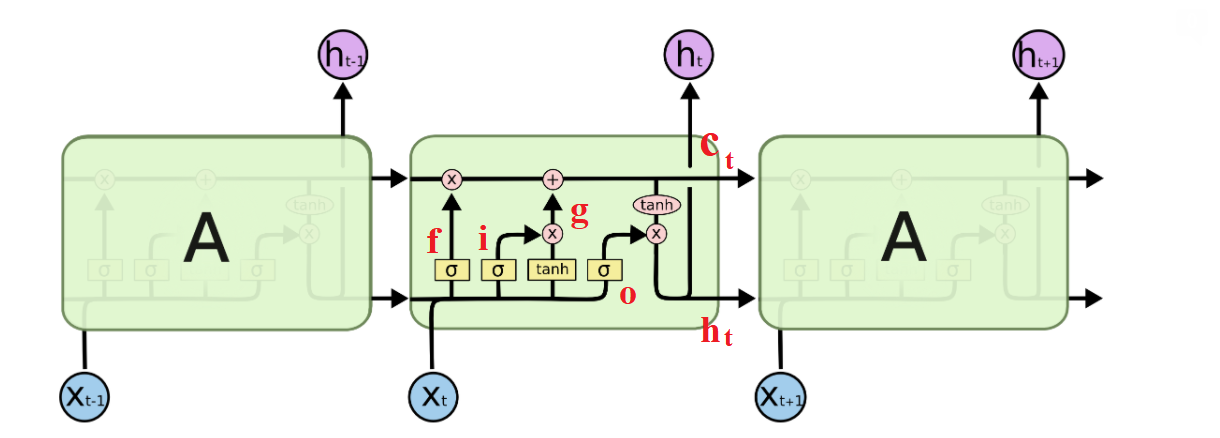
\includegraphics[width=13cm]{LSTM.png}
	\caption{Mô hình LSTM.}
\end{figure} 

Mỗi LSTM cell bao gồm 3 cổng chính \cite{web:6}: 
\begin{itemize}
	\item Forget gate (f):
	Thực hiện việc quyết định thông tin nào từ trước đó sẽ được lưu lại trong bộ nhớ.
	\item Input gate (i):
	Thực hiện việc quyết định những thông tin mới nào sẽ được lưu lại trong bộ nhớ dài hạn.
	\item Output gate (o):
	Thực hiện xem thông tin nào được truyền ra ngoài để phục vụ cho mục đích dự đoán.
\end{itemize}

Ngoài ra thành phần của LSTM cell còn có cell state ($c_t$). Là bộ nhớ trong của LSTM, nó là tổng hợp của bộ nhớ trước $c_{t-1}$ đã được lọc qua Forget gate, cộng với trạng thái ẩn g đã được lọc bởi Input gate sẽ mang thông tin nào quan trọng truyền đi xa hơn và sẽ được dùng khi cần. Đây chính là long term memory.

Cơ chế hoạt động đặc biệt và cổng (gate) của LSTM giúp mô hình có khả năng lưu trữ thông tin dài hạn và xử lý hiệu quả các chuỗi có độ dài khác nhau, giúp khắc phục được các nhược điểm của RNN. Tuy nhiên LSTM vẫn tồn tại điểm yếu là độ phức tạp của nó khiến thời gian xử lý lớn hơn nhiều so với mô hình RNN thông thường.